\section{Results}
% NOTE:
% You are expected to refer to all the floats (figures, tables, etc.)
% in the results section.
Para los resultados fueron necesarios escribirlos dentro un TXT distinto para cada caso y además diferente al que estábamos leyendo dentro de nuestro algoritmo. Dentro de estos TXT de resultados se presentan 3 columnas. La primera columna hace referencia a la cantidad de números que se encuentran dentro del TXT que estamos leyendo. La segunda columna hace referencia a la cantidad de comparaciones realizadas durante todo el algoritmo y finalmente la tercera columna hace referencia al tiempo que se demoró el algoritmo en realizar todo el trabajo solicitado. Posteriormente se presentarán los resultados para los 3 diferentes casos. \\

Mejor Caso:  

Los resultados obtenidos para el mejor caso se presentan donde todos los números dentro del texto son igual a 0, estos resultados se presentan a continuación: 

% shows how to create a table and how to refer to it

\begin{table}[H]	% uses float package to control placement
	\centering	% centers the table
	\caption{
		El número de operaciones y del tiempo transcurrido (nanosegundos) como una función del tamaño de entrada.
	}	% provides a concise description of the table contents

	\begin{tabular}{r r r}
		% table header
		Size & Operations & Elapsed time \\
		% inserts horizontal line
		\hline
		% separates column entries with the ampersand &
		32 & 63 &  3016 \\
		64 & 127 &  2420 \\
		128& 255 &  1456 \\
		256& 511 & 1613 \\
		512& 1023&  2194 \\
	    1024 & 2047 & 4243 \\
	    2048 & 4095 & 7209 \\
	    4096 & 8191 & 12951 \\
	    8192 & 16383 & 27492 \\
	    16384 & 32767 & 50415 \\
	    32768 & 65535 & 96842 \\
	    65536 & 131071 & 191310 \\
	    131072 & 262143 & 390439 \\
	    262144 & 524287 & 766497 \\
	    524288 & 1048575 & 1643614 \\
	    1048576 & 2097151 & 3789424 \\
	        
	\end{tabular}

	% defines a label to refer to it
\end{table}


Una gráfica del número promedio de operaciones y tiempo de ejecución para el mejor caso se muestra en la figure~\ref{fig:best}.

\begin{figure}[H]
	% centers the figure
	\centering
	% my LaTeX installation expects Encapsulated PostScript EPS graphs
	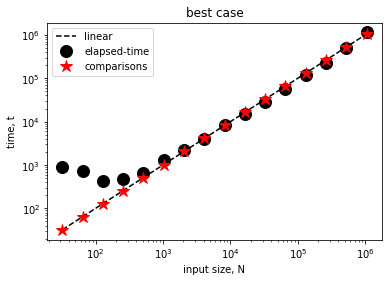
\includegraphics[keepaspectratio, width = 0.75\textwidth]{bestc.png}
	\caption{
		Número promedio de operaciones y tiempo de ejecución como función del tamaño de entrada para el mejor caso.$N$.
	}
	% defines a label to refer to it
	\label{fig:best}
\end{figure}

A primera vista, se puede observar que en un principio los datos no demuestran ningún tipo de comportamiento, pero a medida que se incrementan los datos estos conforman un comportamiento lineal respecto al número de comparaciones realizadas en el algoritmo. 

Caso promedio: 

En este caso ya los números dentro del TXT a leer son completamente aleatorios, ya que son aleatorios se realizaron una menor cantidad de repeticiones y hasta un límite menor de números dentro del TXT a leer. Los resultados se muestran a continuación: 

% shows how to create a table and how to refer to it

\begin{table}[H]	% uses float package to control placement
	\centering	% centers the table
	\caption{
		El número de operaciones y del tiempo transcurrido (nanosegundos) como una función del tamaño de entrada.
	}	% provides a concise description of the table contents

	\begin{tabular}{r r r}
		% table header
		Size & Operations & Elapsed time \\
		% inserts horizontal line
		\hline
		% separates column entries with the ampersand &
		32 & 320 &  2733 \\
		48 & 703 &  1909 \\
		72& 1540 &  3017 \\
		108& 3417 & 4789 \\
		162& 7577&  8642 \\
	    243 & 17013 & 16854 \\
	    364 & 38086 & 34028 \\
	    546 & 84813 & 70789 \\
	    819 & 191679 & 153415 \\
	    1228 & 429594 & 333165 \\
	    1842 & 962638 & 735745 \\
	    2763 & 2169014 & 1616289 \\
	    4144 & 4879156 & 3628981 \\
	        
	\end{tabular}

	% defines a label to refer to it
\end{table}


Una gráfica del número promedio de operaciones y tiempo de ejecución para el caso promedio se muestra en la figure~\ref{fig:best}.

\begin{figure}[H]
	% centers the figure
	\centering
	% my LaTeX installation expects Encapsulated PostScript EPS graphs
	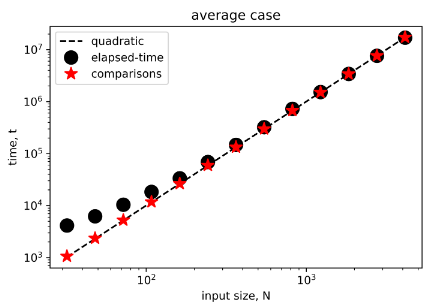
\includegraphics[keepaspectratio, width = 0.75\textwidth]{averagec.png}
	\caption{
		Número promedio de operaciones y tiempo de ejecución como función del tamaño de entrada para el caso promedio.$N^2$.
	}
	% defines a label to refer to it
	\label{fig:best}
\end{figure}
Como se puede observar en la gráfica, el comportamiento de los datos se parece al cuadrático casi desde el principio de la toma de datos. Esto se debe a que es lógico pensar que en un mayor número de comparaciones se va a tomar mayor tiempo realizar el algoritmo. 

Peor caso: 

Dentro del peor caso también se presentan números aleatorios en el TXT a leer, por lo que en la práctica se realiza el mismo procedimiento que para el caso promedio. Los resultados se presentan a continuación: 

% shows how to create a table and how to refer to it

\begin{table}[H]	% uses float package to control placement
	\centering	% centers the table
	\caption{
		El número de operaciones y del tiempo transcurrido (nanosegundos) como una función del tamaño de entrada.
	}	% provides a concise description of the table contents

	\begin{tabular}{r r r}
		% table header
		Size & Operations & Elapsed time \\
		% inserts horizontal line
		\hline
		% separates column entries with the ampersand &
		32 & 528 &  1472 \\
		48 & 1176 &  2286 \\
		72& 2628 &  3731 \\
		108& 5886 & 6795 \\
		162& 13203&  13253 \\
	    243 & 29646 & 26586 \\
	    364 & 66430 & 55426 \\
	    546 & 149331 & 118454 \\
	    819 & 335790 & 260113 \\
	    1228 & 754606 & 574604 \\
	    1842 & 1697403 & 1280200 \\
	    2763 & 2834846 & 2834846 \\
	        
	\end{tabular}

	% defines a label to refer to it
\end{table}


Una gráfica del número promedio de operaciones y tiempo de ejecución para el peor caso se muestra en la figure~\ref{fig:best}.

\begin{figure}[H]
	% centers the figure
	\centering
	% my LaTeX installation expects Encapsulated PostScript EPS graphs
	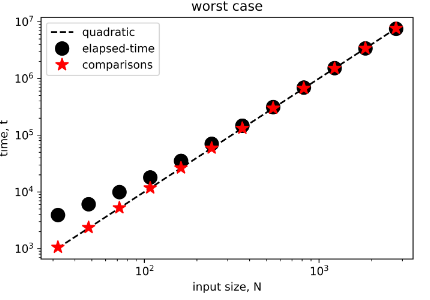
\includegraphics[keepaspectratio, width = 0.75\textwidth]{worstc.png}
	\caption{
		Número promedio de operaciones y tiempo de ejecución como función del tamaño de entrada para el peor caso.$N^2$.
	}
	% defines a label to refer to it
	\label{fig:best}
\end{figure}

Como se puede evidenciar arriba, la gráfica a simple vista se ve muy parecida sino igual al del caso promedio. Estos resultados presentan el mismo comportamiento cuadrático para los datos. 

